% Options for packages loaded elsewhere
\PassOptionsToPackage{unicode}{hyperref}
\PassOptionsToPackage{hyphens}{url}
%
\documentclass[
]{article}
\usepackage{amsmath,amssymb}
\usepackage{lmodern}
\usepackage{ifxetex,ifluatex}
\ifnum 0\ifxetex 1\fi\ifluatex 1\fi=0 % if pdftex
  \usepackage[T1]{fontenc}
  \usepackage[utf8]{inputenc}
  \usepackage{textcomp} % provide euro and other symbols
\else % if luatex or xetex
  \usepackage{unicode-math}
  \defaultfontfeatures{Scale=MatchLowercase}
  \defaultfontfeatures[\rmfamily]{Ligatures=TeX,Scale=1}
\fi
% Use upquote if available, for straight quotes in verbatim environments
\IfFileExists{upquote.sty}{\usepackage{upquote}}{}
\IfFileExists{microtype.sty}{% use microtype if available
  \usepackage[]{microtype}
  \UseMicrotypeSet[protrusion]{basicmath} % disable protrusion for tt fonts
}{}
\makeatletter
\@ifundefined{KOMAClassName}{% if non-KOMA class
  \IfFileExists{parskip.sty}{%
    \usepackage{parskip}
  }{% else
    \setlength{\parindent}{0pt}
    \setlength{\parskip}{6pt plus 2pt minus 1pt}}
}{% if KOMA class
  \KOMAoptions{parskip=half}}
\makeatother
\usepackage{xcolor}
\IfFileExists{xurl.sty}{\usepackage{xurl}}{} % add URL line breaks if available
\IfFileExists{bookmark.sty}{\usepackage{bookmark}}{\usepackage{hyperref}}
\hypersetup{
  pdftitle={Exploring the composition of lithic assemblages in Mesolithic south-eastern Norway},
  pdfauthor={Isak Roalkvam1,},
  hidelinks,
  pdfcreator={LaTeX via pandoc}}
\urlstyle{same} % disable monospaced font for URLs
\usepackage[margin=1in]{geometry}
\usepackage{longtable,booktabs,array}
\usepackage{calc} % for calculating minipage widths
% Correct order of tables after \paragraph or \subparagraph
\usepackage{etoolbox}
\makeatletter
\patchcmd\longtable{\par}{\if@noskipsec\mbox{}\fi\par}{}{}
\makeatother
% Allow footnotes in longtable head/foot
\IfFileExists{footnotehyper.sty}{\usepackage{footnotehyper}}{\usepackage{footnote}}
\makesavenoteenv{longtable}
\usepackage{graphicx}
\makeatletter
\def\maxwidth{\ifdim\Gin@nat@width>\linewidth\linewidth\else\Gin@nat@width\fi}
\def\maxheight{\ifdim\Gin@nat@height>\textheight\textheight\else\Gin@nat@height\fi}
\makeatother
% Scale images if necessary, so that they will not overflow the page
% margins by default, and it is still possible to overwrite the defaults
% using explicit options in \includegraphics[width, height, ...]{}
\setkeys{Gin}{width=\maxwidth,height=\maxheight,keepaspectratio}
% Set default figure placement to htbp
\makeatletter
\def\fps@figure{htbp}
\makeatother
\setlength{\emergencystretch}{3em} % prevent overfull lines
\providecommand{\tightlist}{%
  \setlength{\itemsep}{0pt}\setlength{\parskip}{0pt}}
\setcounter{secnumdepth}{5}
\ifluatex
  \usepackage{selnolig}  % disable illegal ligatures
\fi
\newlength{\cslhangindent}
\setlength{\cslhangindent}{1.5em}
\newlength{\csllabelwidth}
\setlength{\csllabelwidth}{3em}
\newenvironment{CSLReferences}[2] % #1 hanging-ident, #2 entry spacing
 {% don't indent paragraphs
  \setlength{\parindent}{0pt}
  % turn on hanging indent if param 1 is 1
  \ifodd #1 \everypar{\setlength{\hangindent}{\cslhangindent}}\ignorespaces\fi
  % set entry spacing
  \ifnum #2 > 0
  \setlength{\parskip}{#2\baselineskip}
  \fi
 }%
 {}
\usepackage{calc}
\newcommand{\CSLBlock}[1]{#1\hfill\break}
\newcommand{\CSLLeftMargin}[1]{\parbox[t]{\csllabelwidth}{#1}}
\newcommand{\CSLRightInline}[1]{\parbox[t]{\linewidth - \csllabelwidth}{#1}\break}
\newcommand{\CSLIndent}[1]{\hspace{\cslhangindent}#1}

\title{Exploring the composition of lithic assemblages in Mesolithic south-eastern Norway}
\author{Isak Roalkvam\textsuperscript{1,*}}
\date{26 March, 2021}

\begin{document}
\maketitle

{
\setcounter{tocdepth}{2}
\tableofcontents
}
\textsuperscript{1} University of Oslo

\textsuperscript{*} Correspondence: \href{mailto:isak.roalkvam@iakh.uio.no}{Isak Roalkvam \textless{}\href{mailto:isak.roalkvam@iakh.uio.no}{\nolinkurl{isak.roalkvam@iakh.uio.no}}\textgreater{}}

\hypertarget{plots}{%
\section{Plots}\label{plots}}

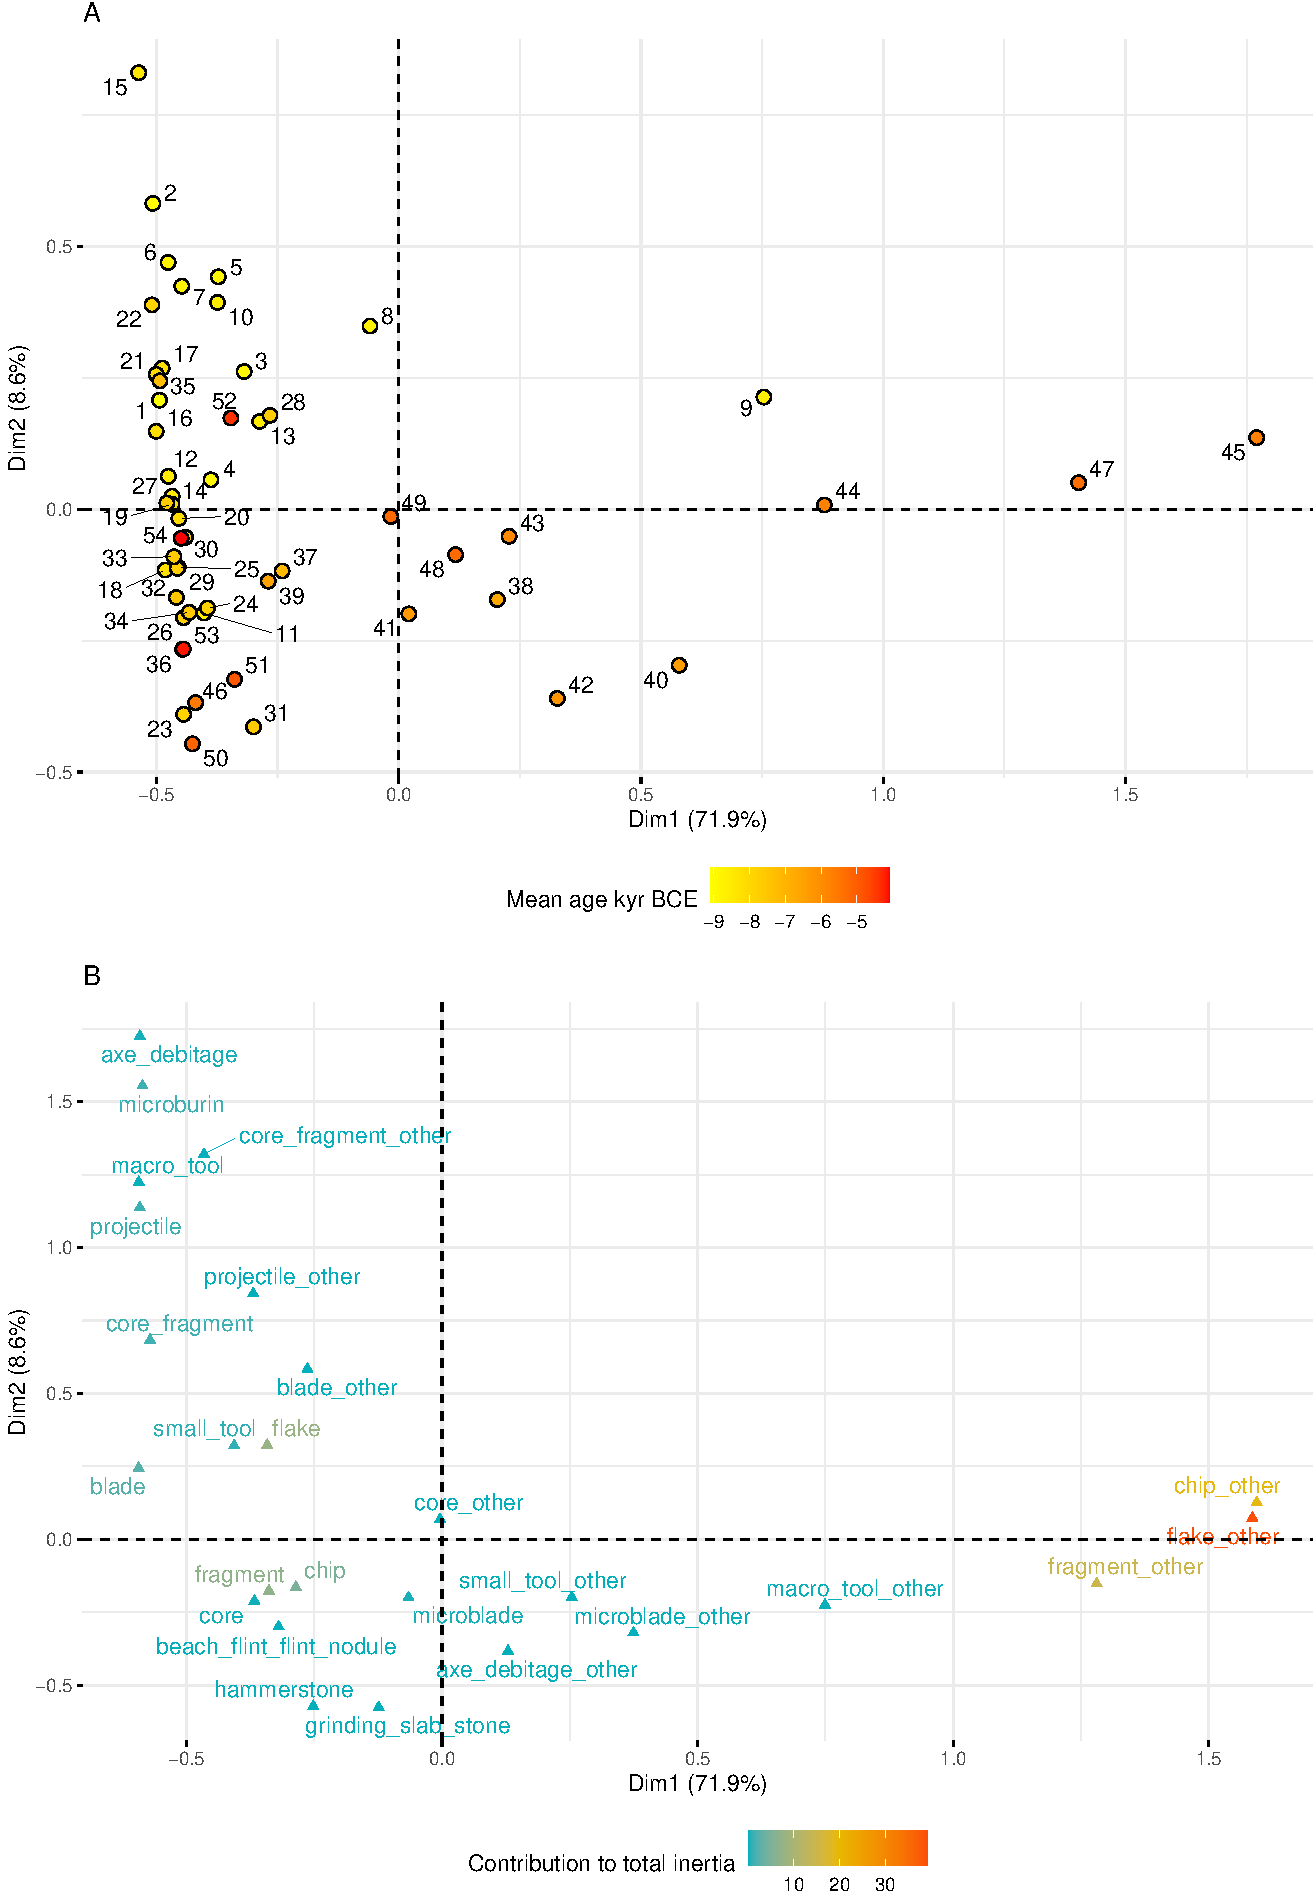
\includegraphics{../figures/cor-1.pdf} 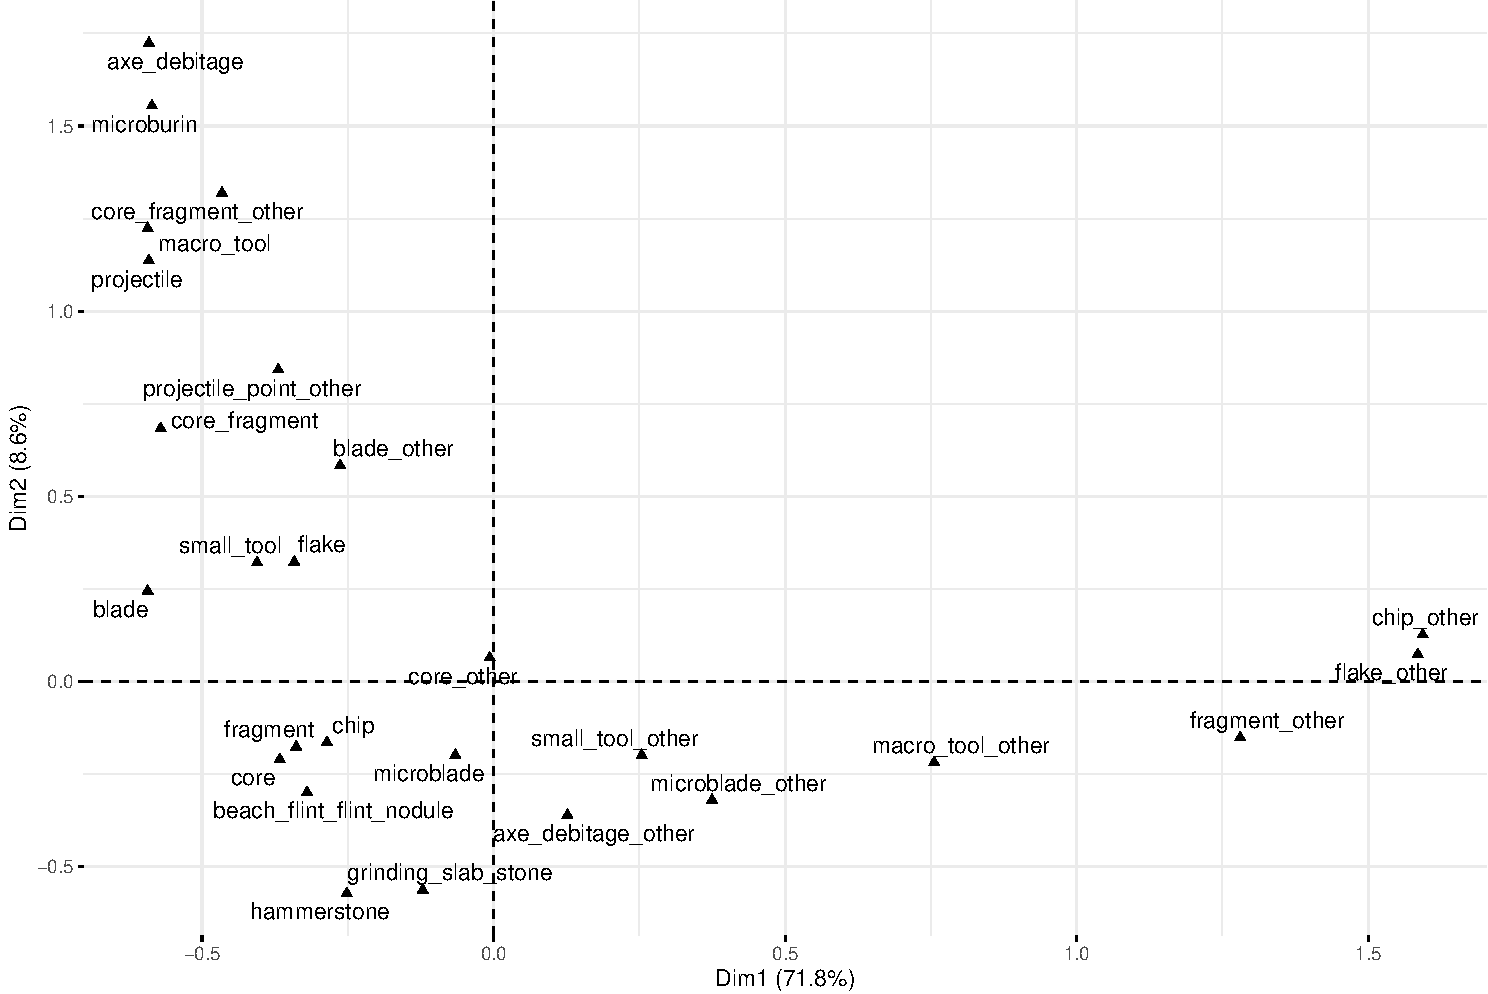
\includegraphics{../figures/cor-2.pdf}

Figure \ref{fig:cor} displays a correspondence analysis using the lithic count data. \ref{fig:cor}

\begin{figure}
\centering
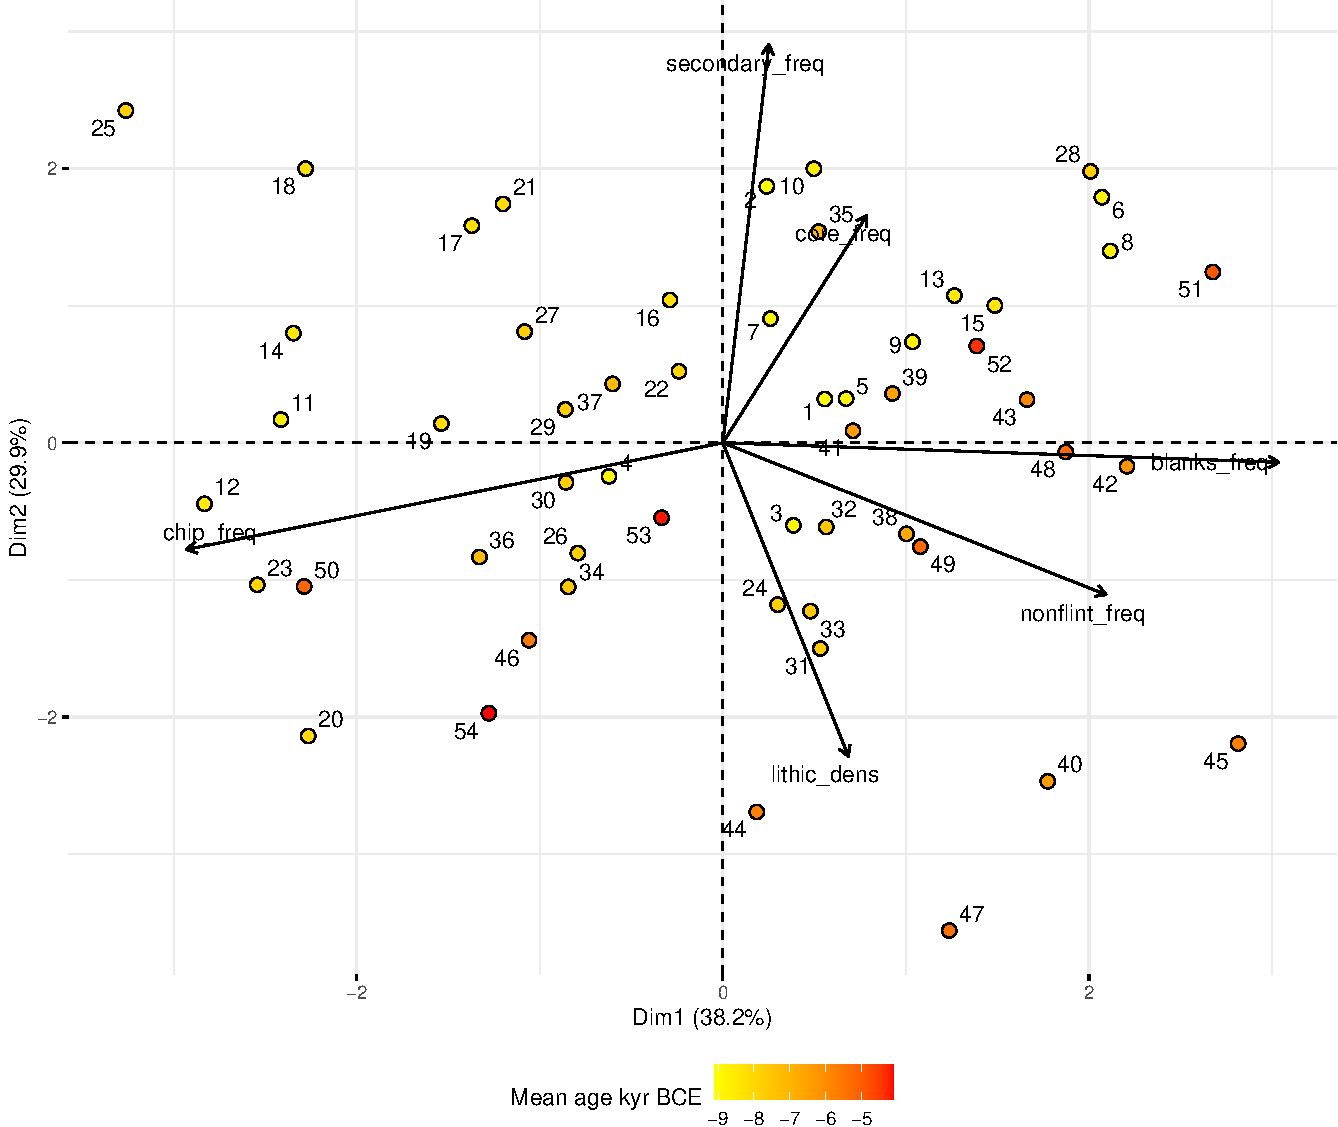
\includegraphics{../figures/pca-analysis-1.pdf}
\caption{\label{fig:pca-analysis}PCA.}
\end{figure}

Figure \ref{fig:pca-analysis} displays a principle components analysis using the continuous measures as defined by Bicho and Cascalheira (2020)

\newpage

\hypertarget{references}{%
\section{References}\label{references}}

\hypertarget{refs}{}
\begin{CSLReferences}{1}{0}
\leavevmode\hypertarget{ref-Bicho2020}{}%
Bicho, N., Cascalheira, J., 2020. Use of lithic assemblages for the definition of short-term occupations in hunter-gatherer prehistory, in: Cascalheira, J., Picin, A. (Eds.),. Springer, Cham, p. 1938. \url{https://doi.org/10.1007/978-3-030-27403-0₂}

\end{CSLReferences}

\newpage

\hypertarget{colophon}{%
\subsubsection{Colophon}\label{colophon}}

This report was generated on 2021-03-26 16:50:59 using the following computational environment and dependencies:

\begin{verbatim}
#> - Session info ---------------------------------------------------------------
#>  setting  value                       
#>  version  R version 4.0.4 (2021-02-15)
#>  os       Linux Mint 19.3             
#>  system   x86_64, linux-gnu           
#>  ui       X11                         
#>  language en_US                       
#>  collate  en_US.UTF-8                 
#>  ctype    en_US.UTF-8                 
#>  tz       Europe/Oslo                 
#>  date     2021-03-26                  
#> 
#> - Packages -------------------------------------------------------------------
#>  package       * version  date       lib source        
#>  abind           1.4-5    2016-07-21 [1] CRAN (R 4.0.3)
#>  assertthat      0.2.1    2019-03-21 [1] CRAN (R 4.0.3)
#>  backports       1.2.0    2020-11-02 [1] CRAN (R 4.0.3)
#>  bookdown        0.21     2020-10-13 [1] CRAN (R 4.0.3)
#>  broom           0.7.3    2020-12-16 [1] CRAN (R 4.0.3)
#>  callr           3.5.1    2020-10-13 [1] CRAN (R 4.0.3)
#>  car             3.0-10   2020-09-29 [1] CRAN (R 4.0.3)
#>  carData         3.0-4    2020-05-22 [1] CRAN (R 4.0.3)
#>  cellranger      1.1.0    2016-07-27 [1] CRAN (R 4.0.3)
#>  cli             2.2.0    2020-11-20 [1] CRAN (R 4.0.3)
#>  cluster         2.1.1    2021-02-14 [4] CRAN (R 4.0.3)
#>  colorspace      1.4-1    2019-03-18 [1] CRAN (R 4.0.3)
#>  crayon          1.3.4    2017-09-16 [1] CRAN (R 4.0.3)
#>  curl            4.3      2019-12-02 [1] CRAN (R 4.0.3)
#>  data.table      1.13.4   2020-12-08 [1] CRAN (R 4.0.3)
#>  DBI             1.1.0    2019-12-15 [1] CRAN (R 4.0.3)
#>  dbplyr          2.0.0    2020-11-03 [1] CRAN (R 4.0.3)
#>  desc            1.2.0    2018-05-01 [1] CRAN (R 4.0.3)
#>  devtools        2.3.2    2020-09-18 [1] CRAN (R 4.0.3)
#>  digest          0.6.27   2020-10-24 [1] CRAN (R 4.0.3)
#>  dplyr         * 1.0.2    2020-08-18 [1] CRAN (R 4.0.3)
#>  DT              0.16     2020-10-13 [1] CRAN (R 4.0.3)
#>  ellipsis        0.3.1    2020-05-15 [1] CRAN (R 4.0.3)
#>  evaluate        0.14     2019-05-28 [1] CRAN (R 4.0.3)
#>  factoextra    * 1.0.7    2020-04-01 [1] CRAN (R 4.0.3)
#>  FactoMineR    * 2.4      2020-12-11 [1] CRAN (R 4.0.3)
#>  fansi           0.4.1    2020-01-08 [1] CRAN (R 4.0.3)
#>  farver          2.0.3    2020-01-16 [1] CRAN (R 4.0.3)
#>  flashClust      1.01-2   2012-08-21 [1] CRAN (R 4.0.3)
#>  forcats       * 0.5.0    2020-03-01 [1] CRAN (R 4.0.3)
#>  foreign         0.8-81   2020-12-22 [4] CRAN (R 4.0.3)
#>  fs              1.5.0    2020-07-31 [1] CRAN (R 4.0.3)
#>  generics        0.1.0    2020-10-31 [1] CRAN (R 4.0.3)
#>  ggplot2       * 3.3.2    2020-06-19 [1] CRAN (R 4.0.3)
#>  ggpubr          0.4.0    2020-06-27 [1] CRAN (R 4.0.3)
#>  ggrepel         0.9.1    2021-01-15 [1] CRAN (R 4.0.3)
#>  ggsignif        0.6.0    2019-08-08 [1] CRAN (R 4.0.3)
#>  glue            1.4.2    2020-08-27 [1] CRAN (R 4.0.3)
#>  gtable          0.3.0    2019-03-25 [1] CRAN (R 4.0.3)
#>  haven           2.3.1    2020-06-01 [1] CRAN (R 4.0.3)
#>  here            1.0.0    2020-11-15 [1] CRAN (R 4.0.3)
#>  highr           0.8      2019-03-20 [1] CRAN (R 4.0.3)
#>  hms             0.5.3    2020-01-08 [1] CRAN (R 4.0.3)
#>  htmltools       0.5.0    2020-06-16 [1] CRAN (R 4.0.3)
#>  htmlwidgets     1.5.2    2020-10-03 [1] CRAN (R 4.0.3)
#>  httr            1.4.2    2020-07-20 [1] CRAN (R 4.0.3)
#>  jsonlite        1.7.1    2020-09-07 [1] CRAN (R 4.0.3)
#>  knitr           1.30     2020-09-22 [1] CRAN (R 4.0.3)
#>  labeling        0.4.2    2020-10-20 [1] CRAN (R 4.0.3)
#>  lattice         0.20-41  2020-04-02 [1] CRAN (R 4.0.3)
#>  leaps           3.1      2020-01-16 [1] CRAN (R 4.0.3)
#>  lifecycle       0.2.0    2020-03-06 [1] CRAN (R 4.0.3)
#>  lubridate       1.7.9.2  2020-11-13 [1] CRAN (R 4.0.3)
#>  magrittr        2.0.1    2020-11-17 [1] CRAN (R 4.0.3)
#>  MASS            7.3-53.1 2021-02-12 [4] CRAN (R 4.0.3)
#>  memoise         1.1.0    2017-04-21 [1] CRAN (R 4.0.3)
#>  modelr          0.1.8    2020-05-19 [1] CRAN (R 4.0.3)
#>  munsell         0.5.0    2018-06-12 [1] CRAN (R 4.0.3)
#>  openxlsx        4.2.3    2020-10-27 [1] CRAN (R 4.0.3)
#>  patchwork     * 1.1.0    2020-11-09 [1] CRAN (R 4.0.3)
#>  pillar          1.4.7    2020-11-20 [1] CRAN (R 4.0.3)
#>  pkgbuild        1.1.0    2020-07-13 [1] CRAN (R 4.0.3)
#>  pkgconfig       2.0.3    2019-09-22 [1] CRAN (R 4.0.3)
#>  pkgload         1.1.0    2020-05-29 [1] CRAN (R 4.0.3)
#>  prettyunits     1.1.1    2020-01-24 [1] CRAN (R 4.0.3)
#>  processx        3.4.4    2020-09-03 [1] CRAN (R 4.0.3)
#>  ps              1.4.0    2020-10-07 [1] CRAN (R 4.0.3)
#>  purrr         * 0.3.4    2020-04-17 [1] CRAN (R 4.0.3)
#>  R6              2.5.0    2020-10-28 [1] CRAN (R 4.0.3)
#>  Rcpp            1.0.5    2020-07-06 [1] CRAN (R 4.0.3)
#>  readr         * 1.4.0    2020-10-05 [1] CRAN (R 4.0.3)
#>  readxl          1.3.1    2019-03-13 [1] CRAN (R 4.0.3)
#>  remotes         2.2.0    2020-07-21 [1] CRAN (R 4.0.3)
#>  reprex          0.3.0    2019-05-16 [1] CRAN (R 4.0.3)
#>  rio             0.5.26   2021-03-01 [1] CRAN (R 4.0.4)
#>  rlang           0.4.10   2020-12-30 [1] CRAN (R 4.0.4)
#>  rmarkdown       2.5      2020-10-21 [1] CRAN (R 4.0.3)
#>  rprojroot       2.0.2    2020-11-15 [1] CRAN (R 4.0.3)
#>  rstatix         0.6.0    2020-06-18 [1] CRAN (R 4.0.3)
#>  rstudioapi      0.13     2020-11-12 [1] CRAN (R 4.0.3)
#>  rvest           0.3.6    2020-07-25 [1] CRAN (R 4.0.3)
#>  scales          1.1.1    2020-05-11 [1] CRAN (R 4.0.3)
#>  scatterplot3d   0.3-41   2018-03-14 [1] CRAN (R 4.0.3)
#>  sessioninfo     1.1.1    2018-11-05 [1] CRAN (R 4.0.3)
#>  stringi         1.5.3    2020-09-09 [1] CRAN (R 4.0.3)
#>  stringr       * 1.4.0    2019-02-10 [1] CRAN (R 4.0.3)
#>  testthat        3.0.0    2020-10-31 [1] CRAN (R 4.0.3)
#>  tibble        * 3.0.4    2020-10-12 [1] CRAN (R 4.0.3)
#>  tidyr         * 1.1.2    2020-08-27 [1] CRAN (R 4.0.3)
#>  tidyselect      1.1.0    2020-05-11 [1] CRAN (R 4.0.3)
#>  tidyverse     * 1.3.0    2019-11-21 [1] CRAN (R 4.0.3)
#>  usethis         2.0.1    2021-02-10 [1] CRAN (R 4.0.4)
#>  vctrs           0.3.5    2020-11-17 [1] CRAN (R 4.0.3)
#>  withr           2.3.0    2020-09-22 [1] CRAN (R 4.0.3)
#>  xfun            0.19     2020-10-30 [1] CRAN (R 4.0.3)
#>  xml2            1.3.2    2020-04-23 [1] CRAN (R 4.0.3)
#>  yaml            2.2.1    2020-02-01 [1] CRAN (R 4.0.3)
#>  zip             2.1.1    2020-08-27 [1] CRAN (R 4.0.3)
#> 
#> [1] /home/isak/R/x86_64-pc-linux-gnu-library/4.0
#> [2] /usr/local/lib/R/site-library
#> [3] /usr/lib/R/site-library
#> [4] /usr/lib/R/library
\end{verbatim}

The current Git commit details are:

\begin{verbatim}
#> Local:    master /home/isak/phd/dialpast_r/dialpastrepository
#> Remote:   master @ origin (https://github.com/isakro/dialpastrepository.git)
#> Head:     [75c1135] 2021-03-26: Initial
\end{verbatim}

\end{document}
